\documentclass[a0,portrait]{a0poster}

\usepackage{multicol} % This is so we can have multiple columns of text side-by-side
\columnsep=100pt % This is the amount of white space between the columns in the poster







\columnseprule=0pt % This is the thickness of the black line between the columns in the poster

\usepackage[svgnames]{xcolor} % Specify colors by their 'svgnames', for a full list of all colors available see here: http://www.latextemplates.com/svgnames-colors

\usepackage{times} % Use the times font
%\usepackage{palatino} % Uncomment to use the Palatino font

\usepackage{dsfont}
\usepackage{tcolorbox}
\usepackage{graphicx} % Required for including images
\graphicspath{{figures/}} % Location of the graphics files
\usepackage{booktabs} % Top and bottom rules for table
\usepackage[font=small,labelfont=bf]{caption} % Required for specifying captions to tables and figures
\usepackage{amsfonts, amsmath, amsthm, amssymb} % For math fonts, symbols and environments
\usepackage{wrapfig} % Allows wrapping text around tables and figures
\usepackage{graphicx}
\usepackage[T1]{fontenc}
\usepackage{lmodern} 

    
\begin{document}

\newcommand{\bra}[1]{\langle #1|}

\newcommand{\ket}[1]{|#1\rangle}

\newcommand{\braket}[2]{\langle #1|#2\rangle}

%----------------------------------------------------------------------------------------
%	POSTER HEADER 
%----------------------------------------------------------------------------------------

% The header is divided into two boxes:
% The first is 75% wide and houses the title, subtitle, names, university/organization and contact information
% The second is 25% wide and houses a logo for your university/organization or a photo of you
% The widths of these boxes can be easily edited to accommodate your content as you see fit

\begin{minipage}[b]{0.75\linewidth}
\veryHuge \color{NavyBlue} \textbf{The General Broken Line Fitter with ATLAS Pixels and Strips} \color{Black}\\ \vspace{1cm} % Title
%\Huge\textit{The General Broken Line Fitter with ATLAS Pixels and Strips}\\[2cm] % Subtitle
\huge \textbf{Alexander Morton}\\[0.5cm] % Author(s)
\huge University of Glasgow, School of Physics \& Astronomy, \\ Partice Physics Experimental\\[0.4cm] % University/organization
\Large \texttt{a.morton.2@research.gla.ac.uk}
\end{minipage}
%
\begin{minipage}[b]{0.25\linewidth}

\includegraphics[width=20cm]{GlaUni.png}\\

\includegraphics[width=7cm]{mp2-logo.png} \hspace{3cm} 
\includegraphics[width=7cm]{gbl-logo.png}\\
\end{minipage}

\vspace{1cm} % A bit of extra whitespace between the header and poster content

%----------------------------------------------------------------------------------------

\begin{multicols}{2} % This is how many columns your poster will be broken into, a portrait poster is generally split into 2 columns

%----------------------------------------------------------------------------------------
%	ABSTRACT
%----------------------------------------------------------------------------------------

\begin{tcolorbox}
\color{Navy} % Navy color for the abstract

\begin{abstract}
The General Broken lines algorithm has bee successfully integrated into the EUTelescope framework. This is designed to be a generic fitter for many different testbeam setups. Many different prototype ATLAS pixel and strip sensors have been taken to the DESY/SLAC testbeam in aid of the upgrade of the ATLAS detector. Results for track fitting and alignment and shown here.


\end{abstract}
\end{tcolorbox}

%----------------------------------------------------------------------------------------
%	INTRODUCTION
%----------------------------------------------------------------------------------------



\begin{tcolorbox}
\color{DarkSlateGray} % DarkSlateGray color for this section

\section*{Background}

\subsection*{Fitting with GBL and Alignment}
Pattern recognition is needed to identify the hits which make up a track. This is dealt with beforehand.
The GBL track fitting and alignment comes in five steps

\begin{itemize}
\item Link GBL points together to form a complete track described by discrete points.
Figure \ref{Scat} shows the linking of GBL point together. It consists of linking measurement/scattering errors using the initial trajectory parametrised.
\item Points which correspond to hits have measurements added with errors. The red points on the green plane of figure \ref{Scat} show these points on the green planes. The measurements pull the track towards it if included in fit.
\item Points with model scattering have kink angles and errors added. The orange points on figure \ref{Scat} show these points. These points allow a kink to be formed relative to the track incidence at that point.
\item Global derivatives which relate motions of the sensors with local frame residuals are added for alignment.
Any relation between the residual on each plane and parameters for the full system. Used in alignment.
\item Local derivatives are added to determine parameters which relate to tracks residual. Useful for kink angle estimations.
\end{itemize}

This information is needed for all track fitting and alignment, apart from the local derivatives. The GBL algorithm is mathematically equivalent to a Kalman filter but computationally different. It solves the above problem in terms of offsets of each GBL point and then relating this back to the usual track parameters. This allows the track solution to be found far more easily

\end{tcolorbox}
\begin{center}
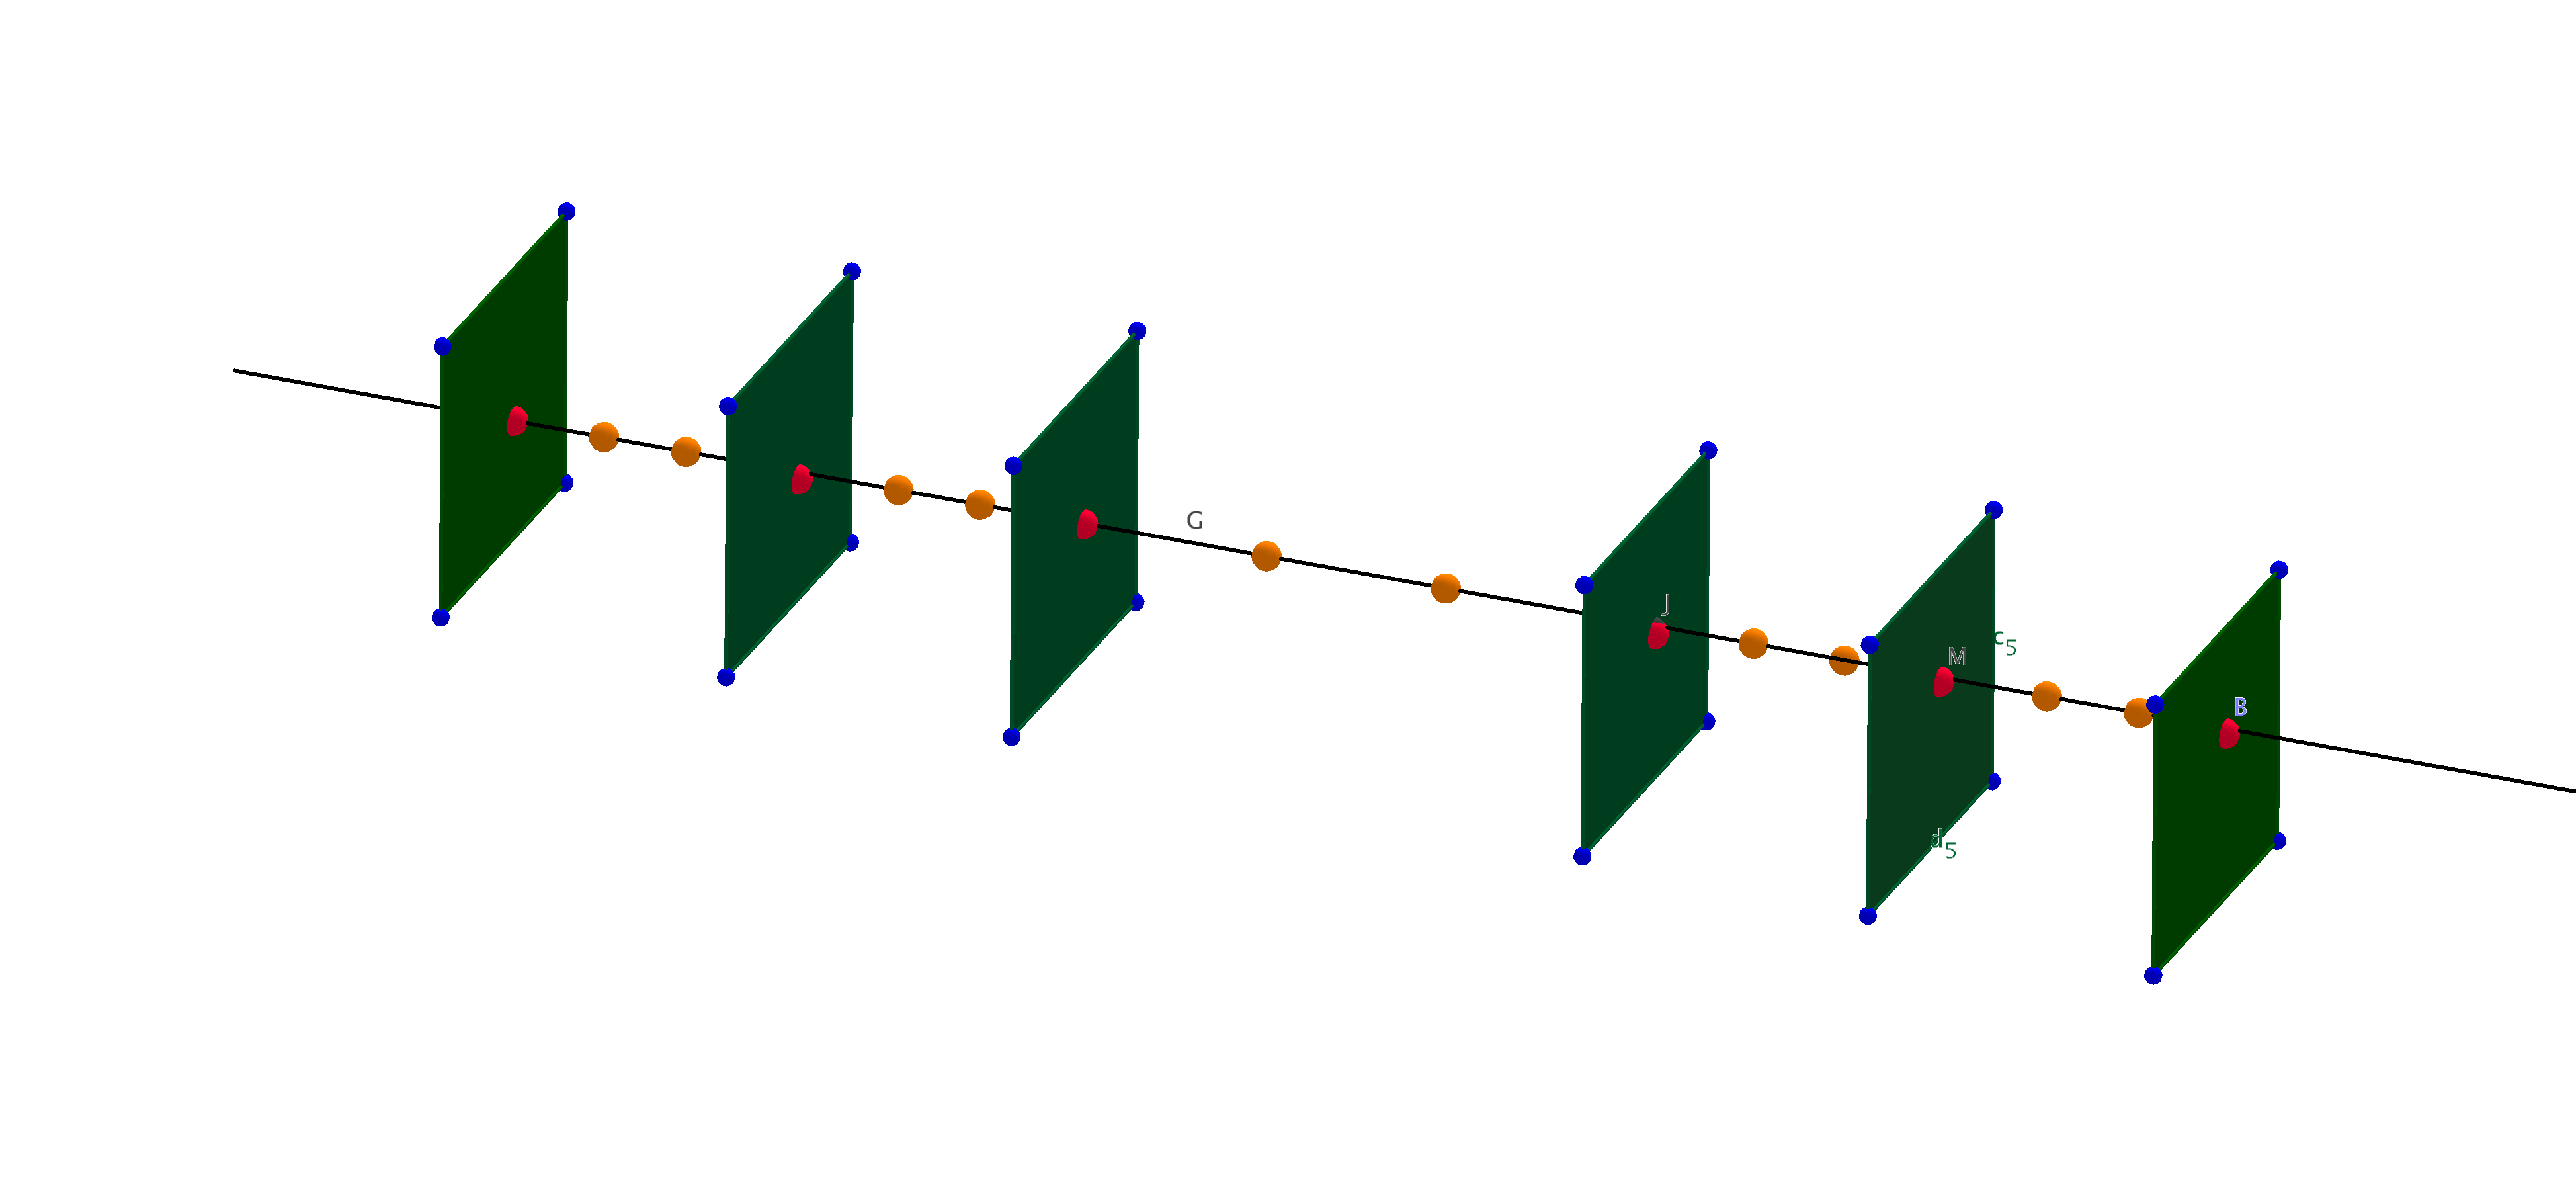
\includegraphics[width=1.0\linewidth]{figures/meas-scat-jac-link.png}
\captionof{figure}{\color{Green} The measurement(red)/scattering(orange) points. All the points are linked together by Jacobians which are determined from the initial trajectory.}
\label{Scat}
\end{center}
\section*{ATLAS Quad module}
\begin{center}
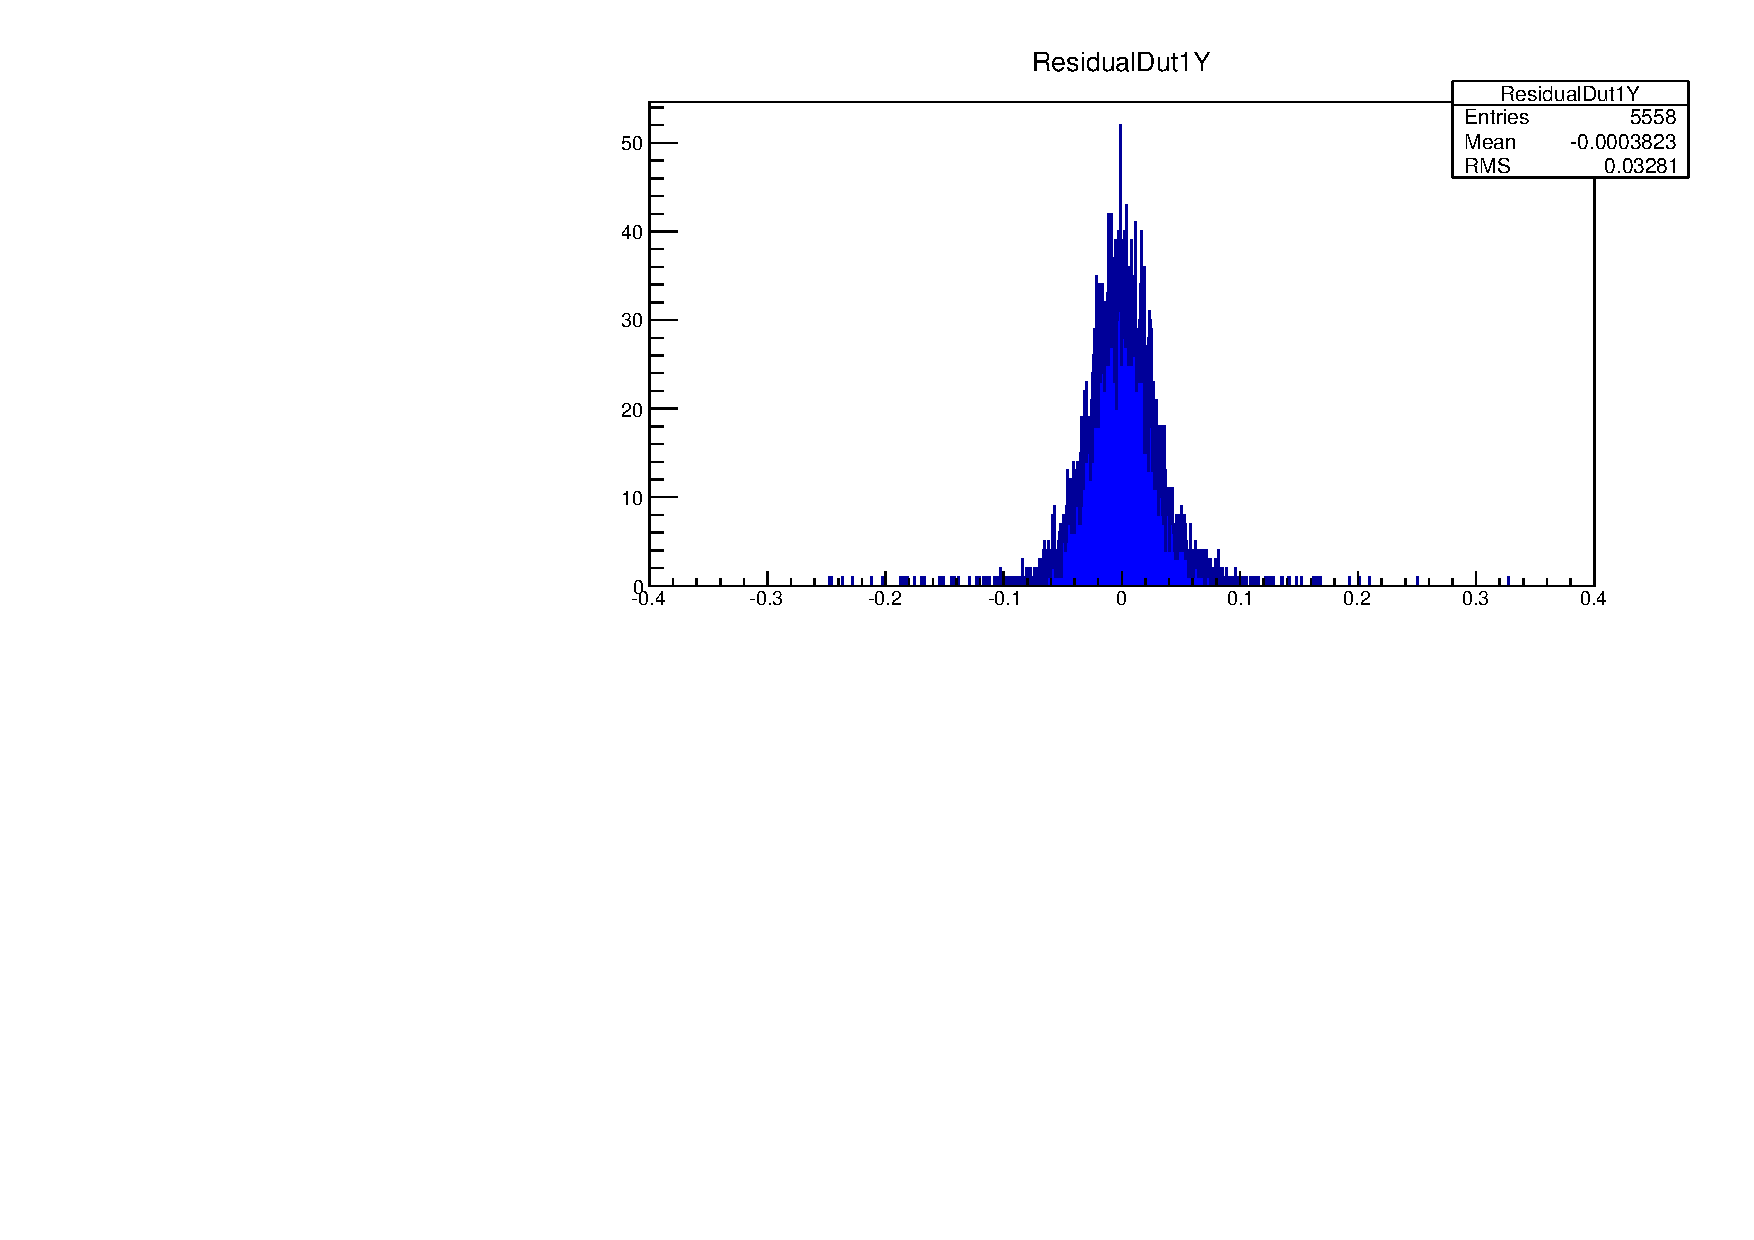
\includegraphics[width=0.8\linewidth]{figures/QuadResY.pdf}
\captionof{figure}{\color{Green} Quad module local Y axis residual for DESY 4 GeV beam}
\label{trine}
\end{center}
ddasd
\section*{ATLAS Pixels}
This setup require a correct description of the scattering for even mimosa sensors due to the DUTs being in a cooling box with high radiation.


\begin{center}
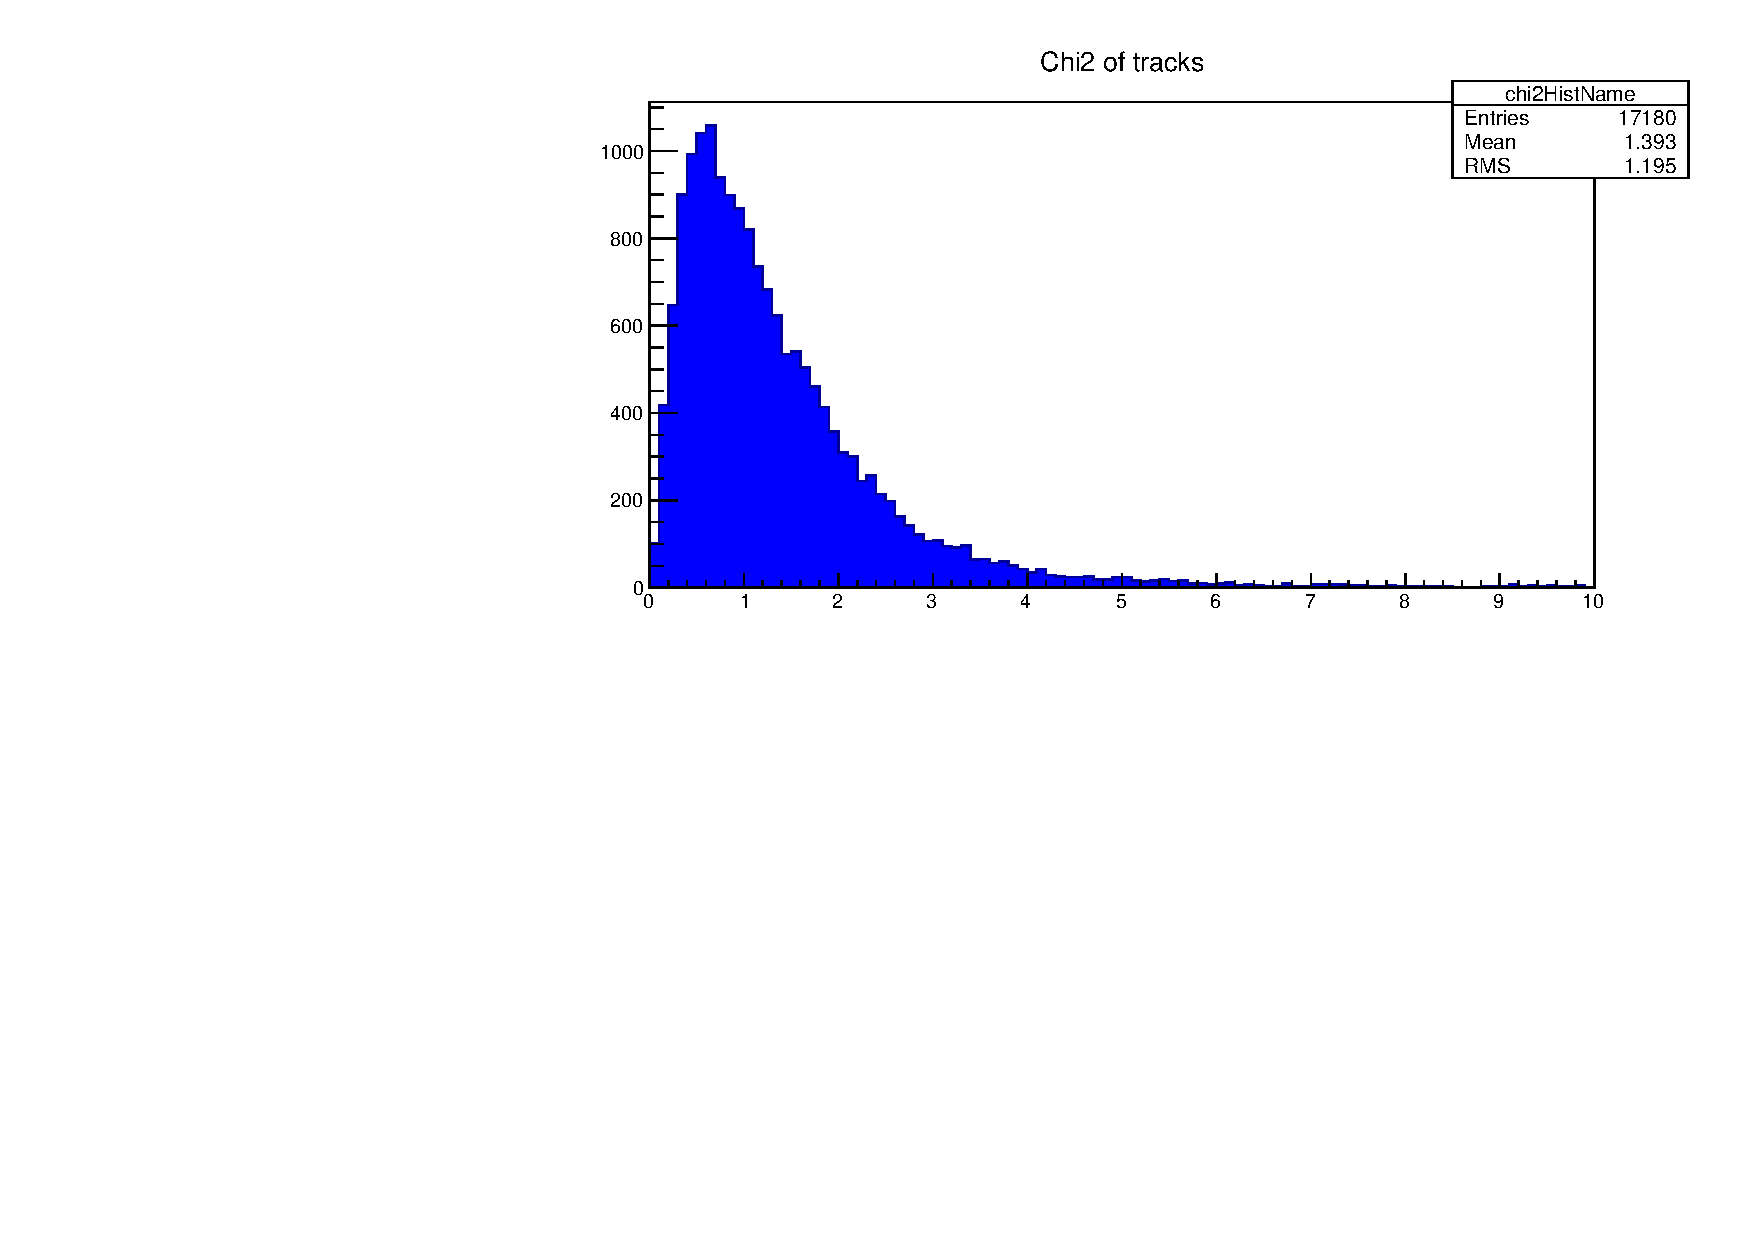
\includegraphics[width=0.7\linewidth]{figures/chi2-313-Corr.pdf}
\captionof{figure}{\color{Green} Chi2/ndf for fit with included radiation length from box. Without inclusion fit does not follow this distribution.}
\label{trine}
\end{center}

\begin{center}
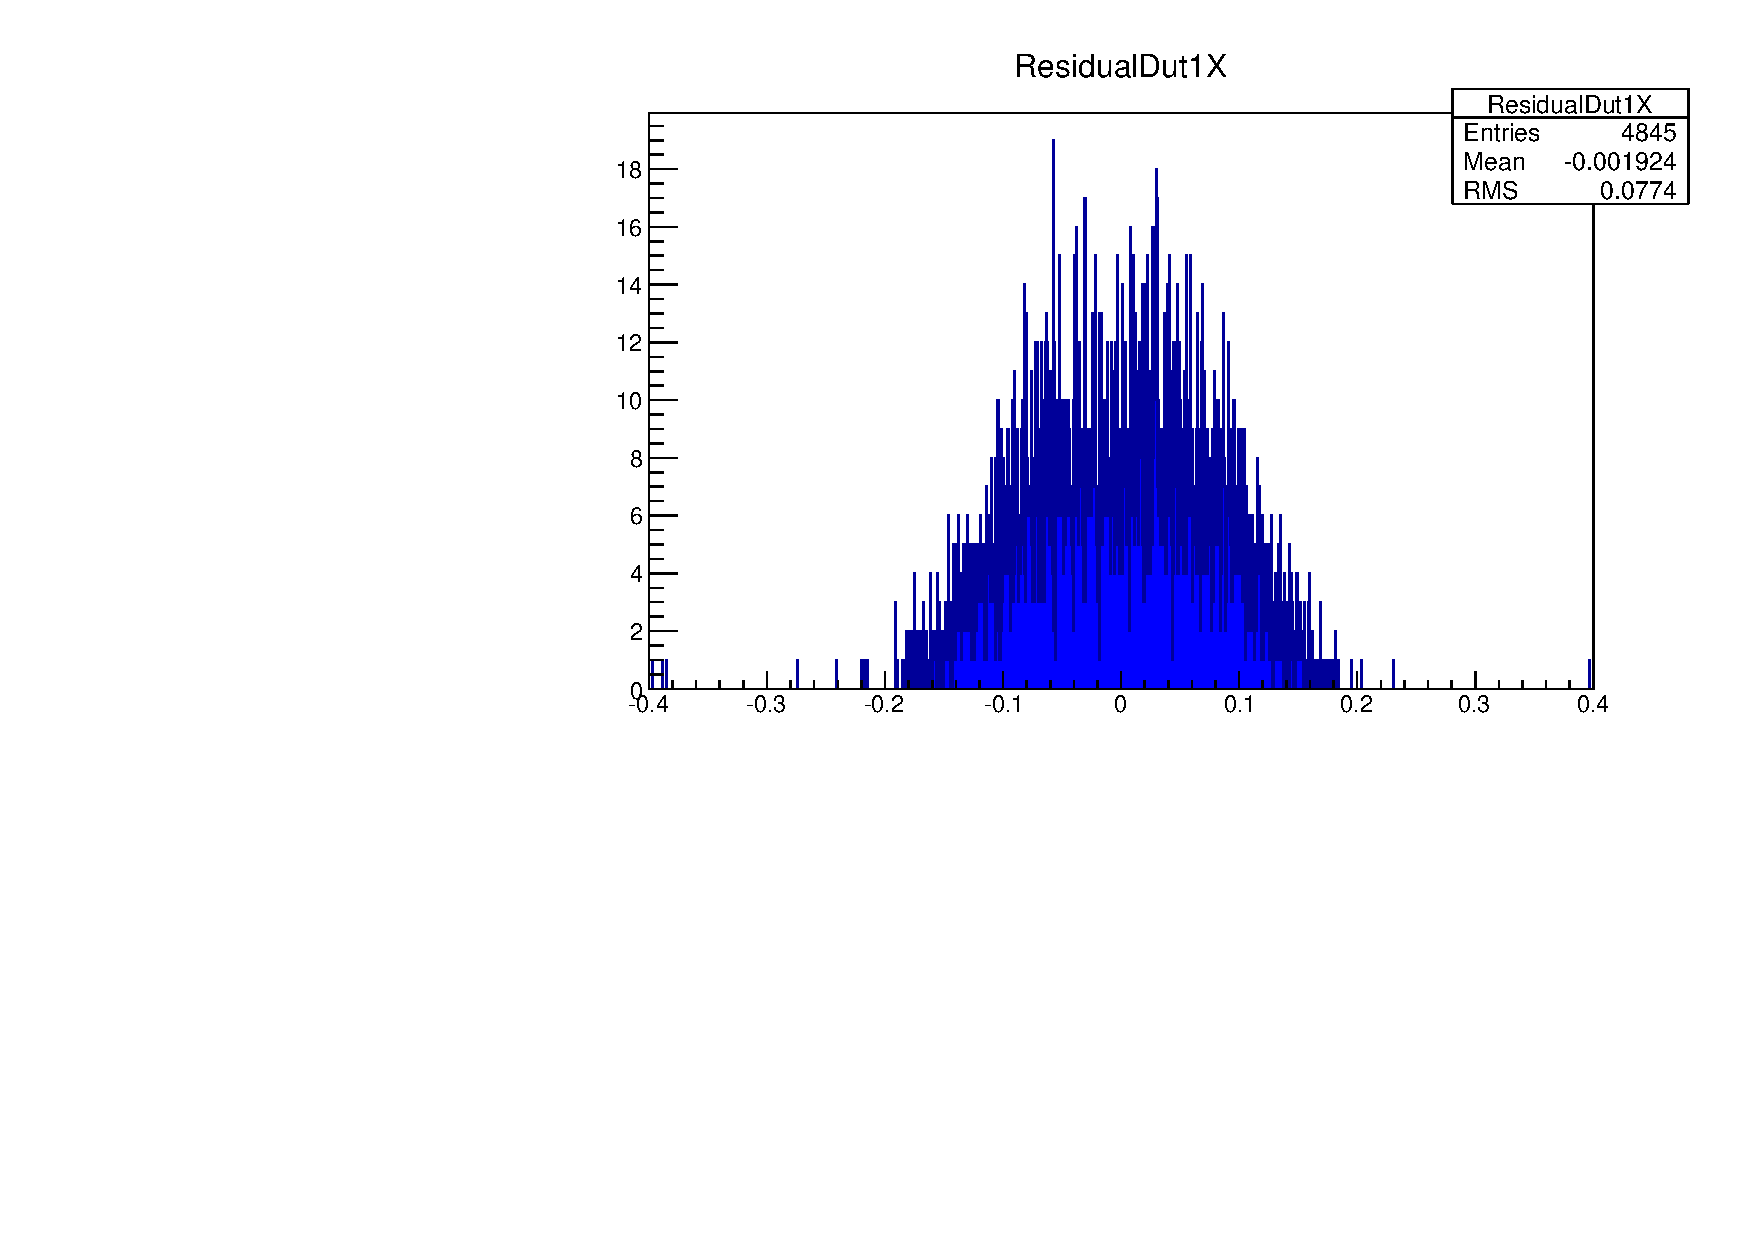
\includegraphics[width=0.7\linewidth]{figures/resXpixel.pdf}
\captionof{figure}{\color{Green} Quad module local Y axis residual for DESY 4 GeV beam}
\label{trine}
\end{center}

\section*{ATLAS strips}
\begin{center}
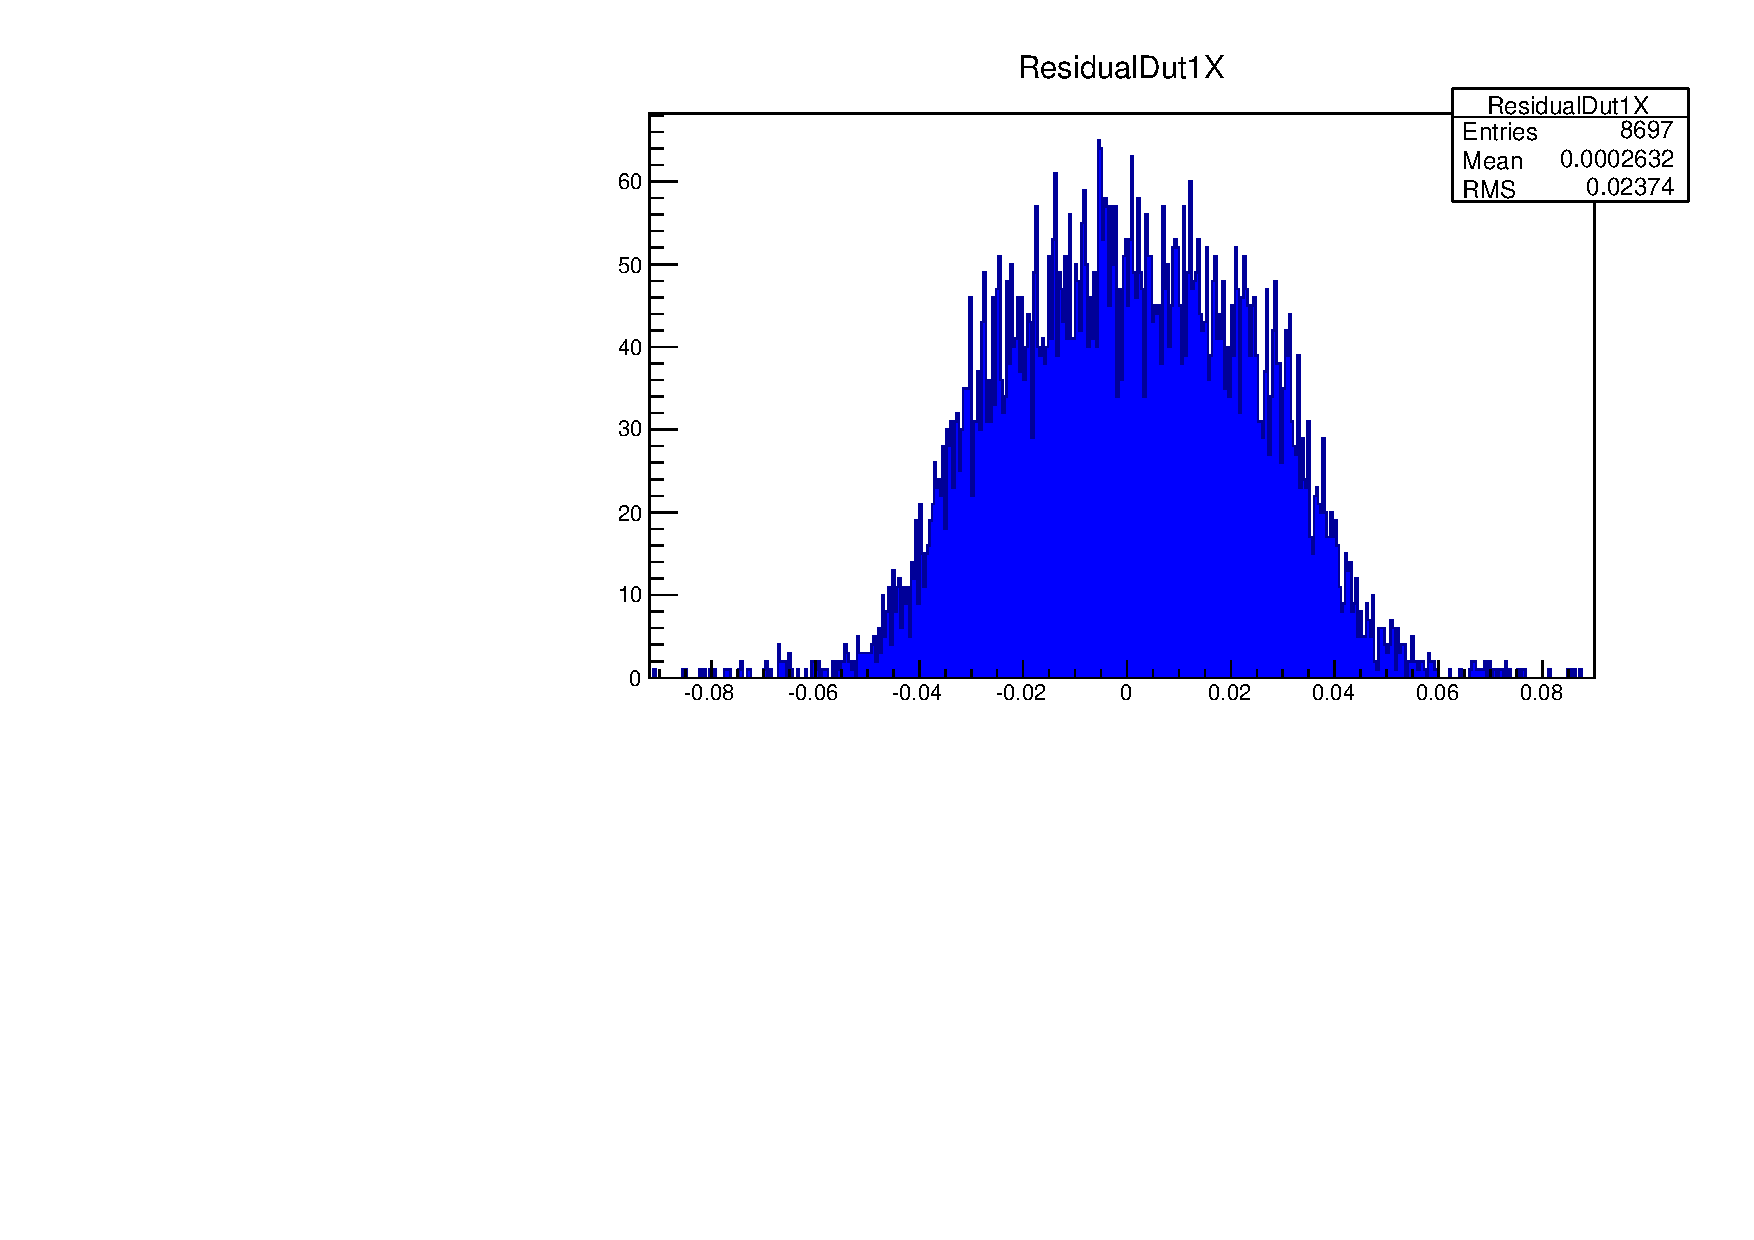
\includegraphics[width=0.7\linewidth]{figures/Res1D.pdf}
\captionof{figure}{\color{Green} Quad module local Y axis residual for DESY 4 GeV beam}
\label{trine}
\end{center}


\section*{Addtonal features}
\subsection*{Magnetic fields}
\begin{center}
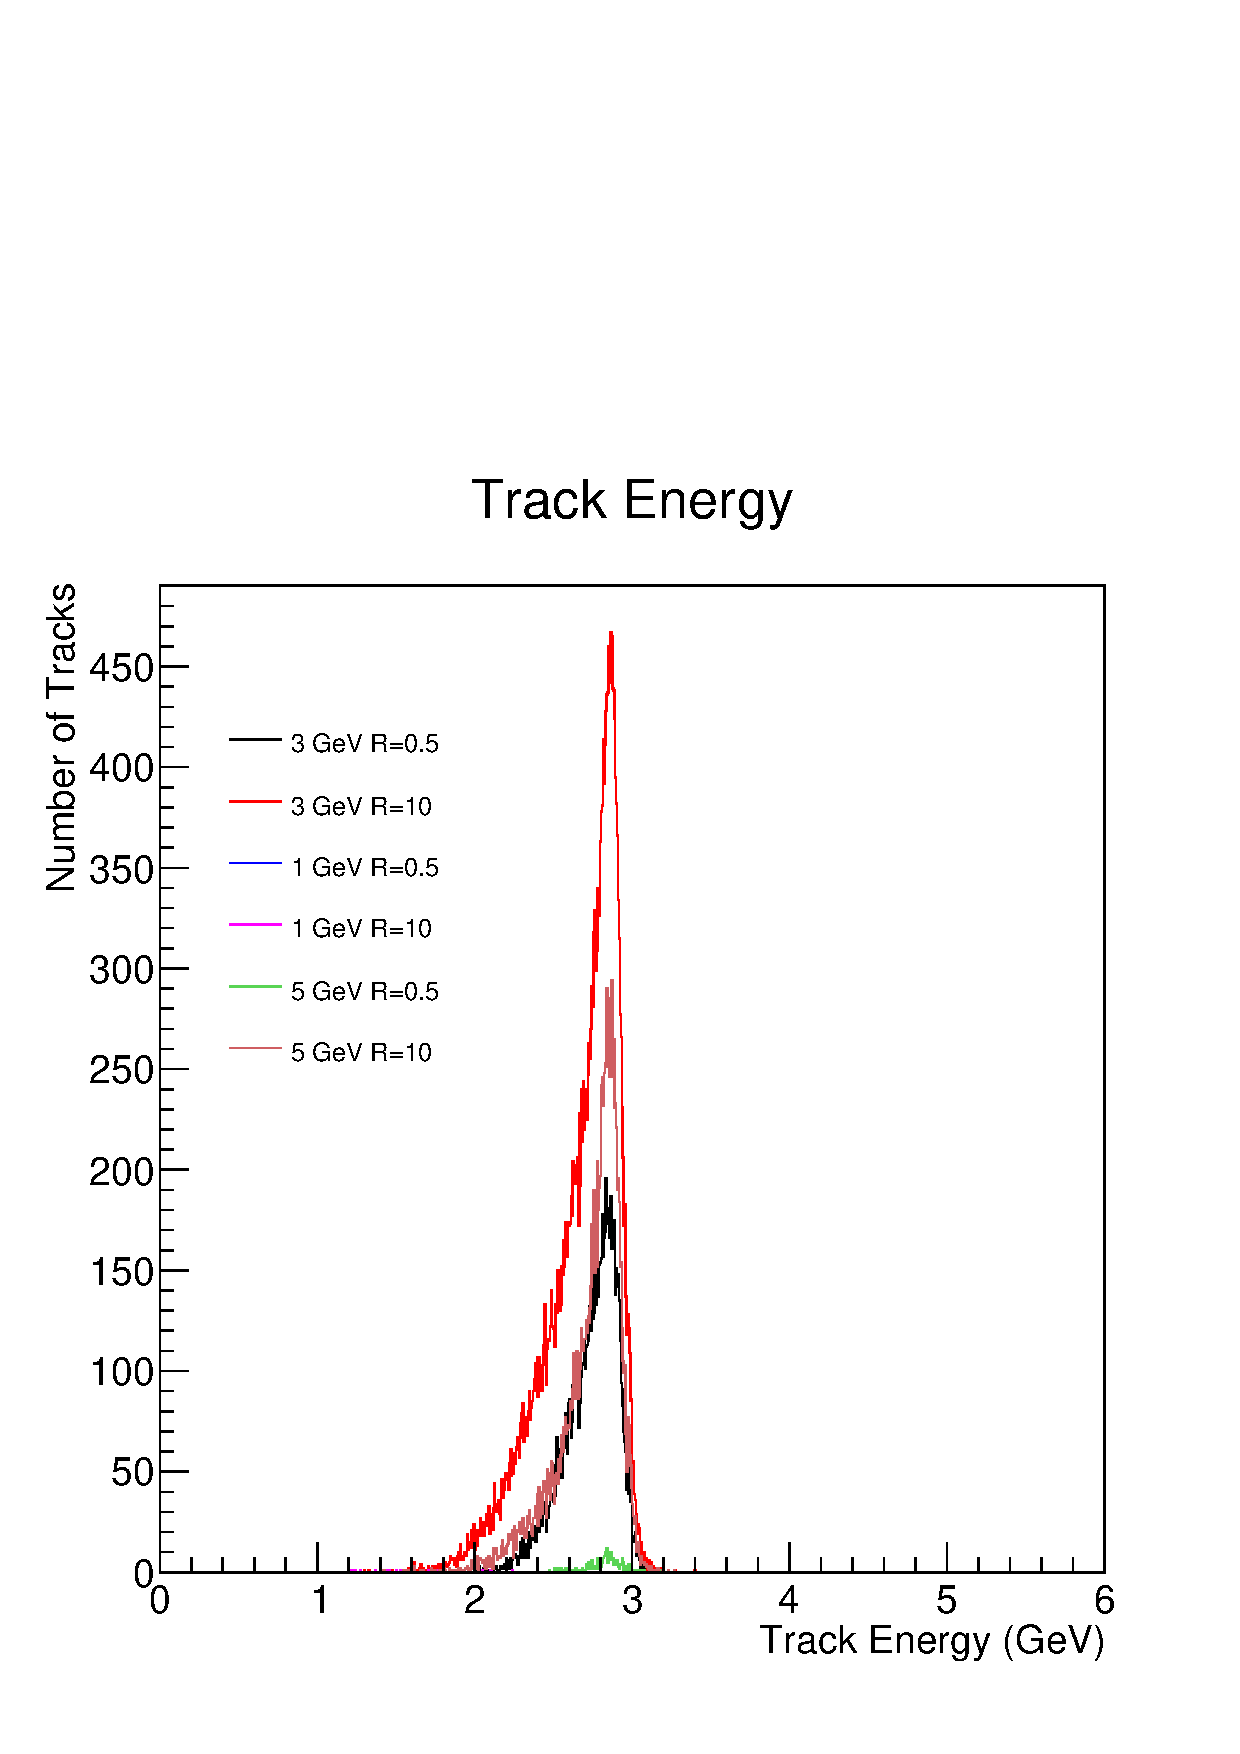
\includegraphics[width=0.8\linewidth]{figures/beamE3B1.pdf}
\captionof{figure}{\color{Green} Measurement of beam energy using the curvature of the beam. Different pattern recognition settings are used to compare possible bias.}
\label{trine}
\end{center}

\subsection*{X0}
\subsection*{Alibava strip}




\begin{thebibliography}{9}
	\bibitem{CheflesCite} Chefles, Anthony, Phys. Lett. A 239 (1998) 339
	\bibitem{Ivanovic} Ivanovic, Igor D. "How to differentiate between non-orthogonal states." Physics Letters A 123.6 (1987): 257-259.
	\bibitem{Dieks} Dieks, Dennis. "Overlap and distinguishability of quantum states." Physics Letters A 126.5 (1988): 303-306.
	\bibitem{Peres} Peres, Asher. "How to differentiate between non-orthogonal states." Physics Letters A 128.1 (1988): 19.
	\bibitem{S&J} Jaeger, Gregg, and Abner Shimony. "Optimal distinction between two non-orthogonal quantum states." Physics Letters A 197.2 (1995): 83-87.
	\bibitem{Sasaki} Sasaki, Masahide, et al. "Accessible information and optimal strategies for real symmetrical quantum sources." Physical Review A 59.5 (1999): 3325.
	\bibitem{Chitambar} Chitambar, Eric, and Min-Hsiu Hsieh. "Revisiting the optimal detection of quantum information." Physical Review A 88.2 (2013): 020302.
\end{thebibliography}

\section*{Acknowledgements}

Thanks to Matthias Sonnleitner, Rob Cameron, Gergely Ferenczi, Va\v{s}ek Poto\v{c}ek \& Thomas Brougham for their help and productive discussions.

%----------------------------------------------------------------------------------------

\end{multicols}
\end{document}
